\section{Design of the PID Controller}\label{designController}
The design of the controller is based on the Root Locus plot, where the final location of the poles in closed loop can be seen. Their position will depend on the different poles, zeros and gain of the controller and that is used to move them to a stable and better location.

As there exists one pole in the Right Half Plane (RHP), the controller must also have one there to create two branches which can be attracted to the Left Half Plane (LHP).

Then, two zeros must be placed in the LHP to make the branches enter in the stable region of the plot.

It is also important for the number of poles to be greater than the number of zeros so that the controller is feasible in reality. This means that two poles need to be placed somewhere so they don't affect the behavior of the final system. This can be achieved if they are placed in the LHP and far from the imaginary axis.

Finally, the gain must be adjusted to make the closed loop poles to be in a stable location. The resultant Root Locus can be seen in \figref{RLControllerZoom}.

\begin{figure}[H]
	\centering 
	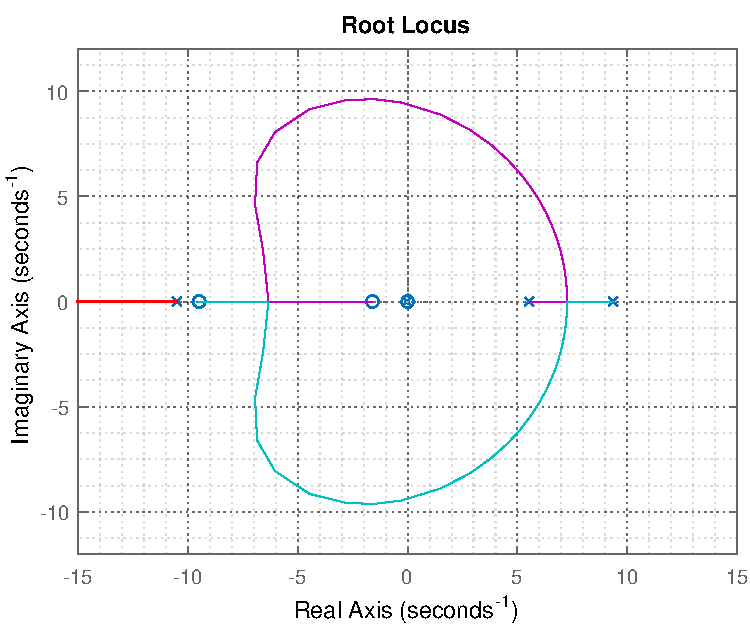
\includegraphics[scale=.56]{figures/RLControllerZoom}
	\captionof{figure}{Root Locus of the final system}
	\label{RLControllerZoom}
\end{figure}
%
The final system looks like \figref{blockDiagramController} and the transfer function of the controller is give by \eqref{ControllerLaplace}.
%
\begin{figure}[H]
	\begin{tikzpicture}[ auto,
thick,                         %<--setting line style
node distance=1.5cm,             %<--setting default node distance
scale=0.75,                     %<--|these two scale the whole thing
every node/.style={scale=0.62}, %<  |(always change both)
>=triangle 45 ]

%-- Blocks creation --%
\draw
% DIRECT TERM %
node[shape=coordinate][](input1) at (0,0){}
node[shape=coordinate][](feed) at (0.5,0){}
node(sum1) at (2,0) [sum] {$\sum$}
node(controller) at (4,0) [block]{\Large $D(s)$}
node(plant) at (6,0) [block]{\Large $G(s)$}
node[shape=coordinate][](DummyNode) at (5,-1.5){}
node[shape=coordinate][](FeedbackNode) at (7.5,0){}
;

%-- Block linking --%
% INPUT %
\draw[-](input1)        -- node{\Large $U(s)$}(feed);
\draw[->](feed)  -- (sum1);

% OUTPUT %
\draw[-](plant)  -- (FeedbackNode);
\draw[->](FeedbackNode)       -- node {\Large $Y(s)$} (9,0);

% DIRECT TERM %
\draw[->] (sum1)            -- (controller);
\draw[->] (controller)       -- (plant);

% FEEDBACKS %
\draw[-] (FeedbackNode)  |- (DummyNode);
\draw[->] (DummyNode)  -| (sum1);

%-- Nodes --%
\draw%--------------------------------------------------------------
node at (input1)            [shift={(-0.04, -0.05 )}] {\Large \textopenbullet}
node at (FeedbackNode)      [shift={(0, -0.07 )}] {\Large \textbullet}
;
%-- Summation signs --%
\draw%--------------------------------------------------------------
node at (sum1) [right = -6.6mm, below = .6mm] {$+$}
node at (sum1) [right = -3mm, below = 3.9mm]  {$-$}
;

\end{tikzpicture} 
	\centering
	\caption{Block diagram of the system}
	\label{blockDiagramController}
\end{figure}
%
\begin{flalign}
	\eq{D(s)} {0,62737 \cdot \frac{(0,1054\ s + 1)\cdot (0,6254\ s + 1)}{(0,1805\ s - 1) \cdot (0,01\ s + 1) \cdot (0,005\ s + 1)}} & \nonumber\\
	\label{ControllerLaplace}
\end{flalign}
%
The stability of the controlled system can be then analyzed using the Nyquist plot of the controller and the plant together in open loop, as seen in \figref{nyquistController}.

\begin{figure}[H] 
	\centering 
	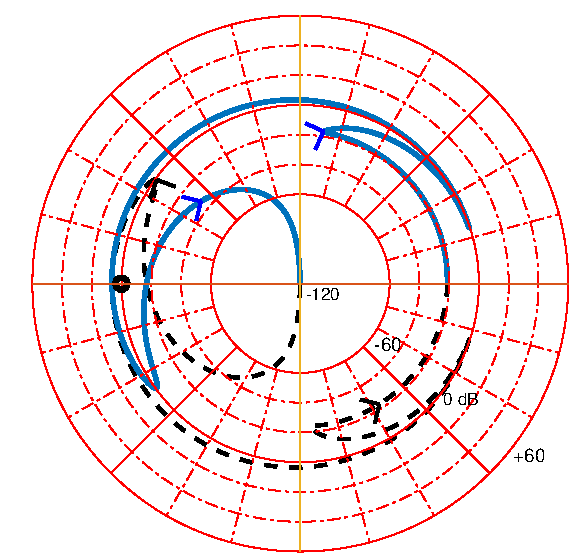
\includegraphics[scale=0.46]{figures/nyquistController}	
	\caption{Nyquist plot of the system with the controller}
	\label{nyquistController}
\end{figure}

Now there are two poles in the RHP and the number of encirclements around -1 equals -2 (they are counterclockwise). 
This means that the system is stable, as the number of zeros in the RHP becomes 0, (see \secref{sec:stabilityAnalysis}).